% Options for packages loaded elsewhere
\PassOptionsToPackage{unicode}{hyperref}
\PassOptionsToPackage{hyphens}{url}
%
\documentclass[
  ignorenonframetext,
]{beamer}
\usepackage{pgfpages}
\setbeamertemplate{caption}[numbered]
\setbeamertemplate{caption label separator}{: }
\setbeamercolor{caption name}{fg=normal text.fg}
\beamertemplatenavigationsymbolsempty
% Prevent slide breaks in the middle of a paragraph
\widowpenalties 1 10000
\raggedbottom
\setbeamertemplate{part page}{
  \centering
  \begin{beamercolorbox}[sep=16pt,center]{part title}
    \usebeamerfont{part title}\insertpart\par
  \end{beamercolorbox}
}
\setbeamertemplate{section page}{
  \centering
  \begin{beamercolorbox}[sep=12pt,center]{part title}
    \usebeamerfont{section title}\insertsection\par
  \end{beamercolorbox}
}
\setbeamertemplate{subsection page}{
  \centering
  \begin{beamercolorbox}[sep=8pt,center]{part title}
    \usebeamerfont{subsection title}\insertsubsection\par
  \end{beamercolorbox}
}
\AtBeginPart{
  \frame{\partpage}
}
\AtBeginSection{
  \ifbibliography
  \else
    \frame{\sectionpage}
  \fi
}
\AtBeginSubsection{
  \frame{\subsectionpage}
}
\usepackage{lmodern}
\usepackage{amssymb,amsmath}
\usepackage{ifxetex,ifluatex}
\ifnum 0\ifxetex 1\fi\ifluatex 1\fi=0 % if pdftex
  \usepackage[T1]{fontenc}
  \usepackage[utf8]{inputenc}
  \usepackage{textcomp} % provide euro and other symbols
\else % if luatex or xetex
  \usepackage{unicode-math}
  \defaultfontfeatures{Scale=MatchLowercase}
  \defaultfontfeatures[\rmfamily]{Ligatures=TeX,Scale=1}
\fi
\usetheme[]{Berlin}
% Use upquote if available, for straight quotes in verbatim environments
\IfFileExists{upquote.sty}{\usepackage{upquote}}{}
\IfFileExists{microtype.sty}{% use microtype if available
  \usepackage[]{microtype}
  \UseMicrotypeSet[protrusion]{basicmath} % disable protrusion for tt fonts
}{}
\makeatletter
\@ifundefined{KOMAClassName}{% if non-KOMA class
  \IfFileExists{parskip.sty}{%
    \usepackage{parskip}
  }{% else
    \setlength{\parindent}{0pt}
    \setlength{\parskip}{6pt plus 2pt minus 1pt}}
}{% if KOMA class
  \KOMAoptions{parskip=half}}
\makeatother
\usepackage{xcolor}
\IfFileExists{xurl.sty}{\usepackage{xurl}}{} % add URL line breaks if available
\IfFileExists{bookmark.sty}{\usepackage{bookmark}}{\usepackage{hyperref}}
\hypersetup{
  pdftitle={Welcome Home --- Now Vote!},
  pdfauthor={Kevin Morris},
  hidelinks,
  pdfcreator={LaTeX via pandoc}}
\urlstyle{same} % disable monospaced font for URLs
\newif\ifbibliography
\setlength{\emergencystretch}{3em} % prevent overfull lines
\providecommand{\tightlist}{%
  \setlength{\itemsep}{0pt}\setlength{\parskip}{0pt}}
\setcounter{secnumdepth}{-\maxdimen} % remove section numbering
\newlength{\cslhangindent}
\setlength{\cslhangindent}{1.5em}
\newenvironment{cslreferences}%
  {\setlength{\parindent}{0pt}%
  \everypar{\setlength{\hangindent}{\cslhangindent}}\ignorespaces}%
  {\par}

\title{Welcome Home --- Now Vote!}
\subtitle{Voting Rights Restoration and Post-Supervision Turnout}
\author{Kevin Morris}
\date{Midwest Political Science Association, 2020}
\institute{Brennan Center for Justice}

\begin{document}
\frame{\titlepage}
\begin{abstract}
\href{mailto:kevin.morris@nyu.edu}{\nolinkurl{kevin.morris@nyu.edu}}
\end{abstract}

\begin{frame}{Outline}
\protect\hypertarget{outline}{}
\begin{itemize}[<+->]
\tightlist
\item
  Previous research indicates that notification laws increase
  post-supervision turnout
\end{itemize}

\begin{itemize}[<+->]
\tightlist
\item
  The notification laws are ``baked in'' to the control group here. In
  2018, New York State began implementing rights restoration prior to
  parole discharge at in-person meetings.
\end{itemize}

\begin{itemize}[<+->]
\tightlist
\item
  So --- did rights restoration \emph{prior} to parole discharge
  increase formerly incarcerated individuals' propensity to vote?
\end{itemize}
\end{frame}

\begin{frame}{Formerly Incarcerated Individuals Turn Out at Low Rates}
\protect\hypertarget{formerly-incarcerated-individuals-turn-out-at-low-rates}{}
\begin{itemize}[<+->]
\tightlist
\item
  The low turnout rates among the formerly disenfranchised have been
  shown in a number of studies (e.g.~Burch 2011, 2012; White 2019)
\end{itemize}

\begin{itemize}[<+->]
\tightlist
\item
  The \emph{causal effect} of incarceration, however, is the subject of
  some debate. Gerber et al. (2017), for instance, argues that most of
  the low turnout observed in the formerly incarcerated population is
  attributable not to incarceration, but to other factors predating
  incarceration.
\end{itemize}

\begin{itemize}[<+->]
\tightlist
\item
  Nevertheless, Lerman and Weaver (2014) and others have convincingly
  shown through qualitative and quantitative work that criminal justice
  involvement structures individuals' relationship to the state.
\end{itemize}
\end{frame}

\begin{frame}{Notification Laws and Post-Supervision Turnout}
\protect\hypertarget{notification-laws-and-post-supervision-turnout}{}
\begin{itemize}[<+->]
\tightlist
\item
  In 2005, Iowa changed its disenfranchisement laws to allow formerly
  incarcerated individuals to vote. Not all formerly incarcerated
  individuals, however, were notified of the change in the mail.
  Meredith and Morse (2015) exploits this uneven treatment,
  demonstrating that mail notification increased turnout.
\end{itemize}

\begin{itemize}[<+->]
\tightlist
\item
  In 2012, Gerber et al. (2015) expanded on the natural experiment setup
  of Meredith and Morse (2015). In a randomized experiment, they sent
  mail notifications to some formerly disenfranchised individuals in
  Connecticut. They too find that notification increases participation,
  arguing ``Whatever the participatory consequences of incarceration
  they are not in large part impossible to overcome'' (p.~924).
\end{itemize}
\end{frame}

\begin{frame}{Changes in New York State in 2018}
\protect\hypertarget{changes-in-new-york-state-in-2018}{}
\begin{itemize}[<+->]
\tightlist
\item
  In the spring of 2018, Governor Andrew Cuomo signs Executive Order 181
  restoring voting rights to individuals \emph{prior} to their discharge
  from parole.
\end{itemize}

\begin{itemize}[<+->]
\tightlist
\item
  The New York DOC issues guidance calling the program a \emph{priority}
  initiative, telling parole officers to help their parolees register to
  vote.
\end{itemize}

\begin{itemize}[<+->]
\tightlist
\item
  Does in-person rights restoration prior to parole discharge increase
  post-supervision turnout?
\end{itemize}
\end{frame}

\begin{frame}{Methodology}
\protect\hypertarget{methodology}{}
\begin{itemize}[<+->]
\tightlist
\item
  I limit the pool of individuals to those discharged before the 2018
  registration deadline in 2018. These are all individuals, therefore,
  who could have voted even if the executive order had not been
  implemented.
\end{itemize}

\begin{itemize}[<+->]
\tightlist
\item
  I compare turnout to those treated by the executive order to those who
  were untreated by the order afterwards.
\end{itemize}

\begin{itemize}[<+->]
\tightlist
\item
  Because of ``imperfect compliance'' with the treatment, I adopt an
  instrumental variables approach. Treatment is instrumented by whether
  someone came off parole after the executive order went into effect.
\end{itemize}
\end{frame}

\begin{frame}{Turnout in 2016 Among the Formerly Incarcerated}
\protect\hypertarget{turnout-in-2016-among-the-formerly-incarcerated}{}
\begin{center}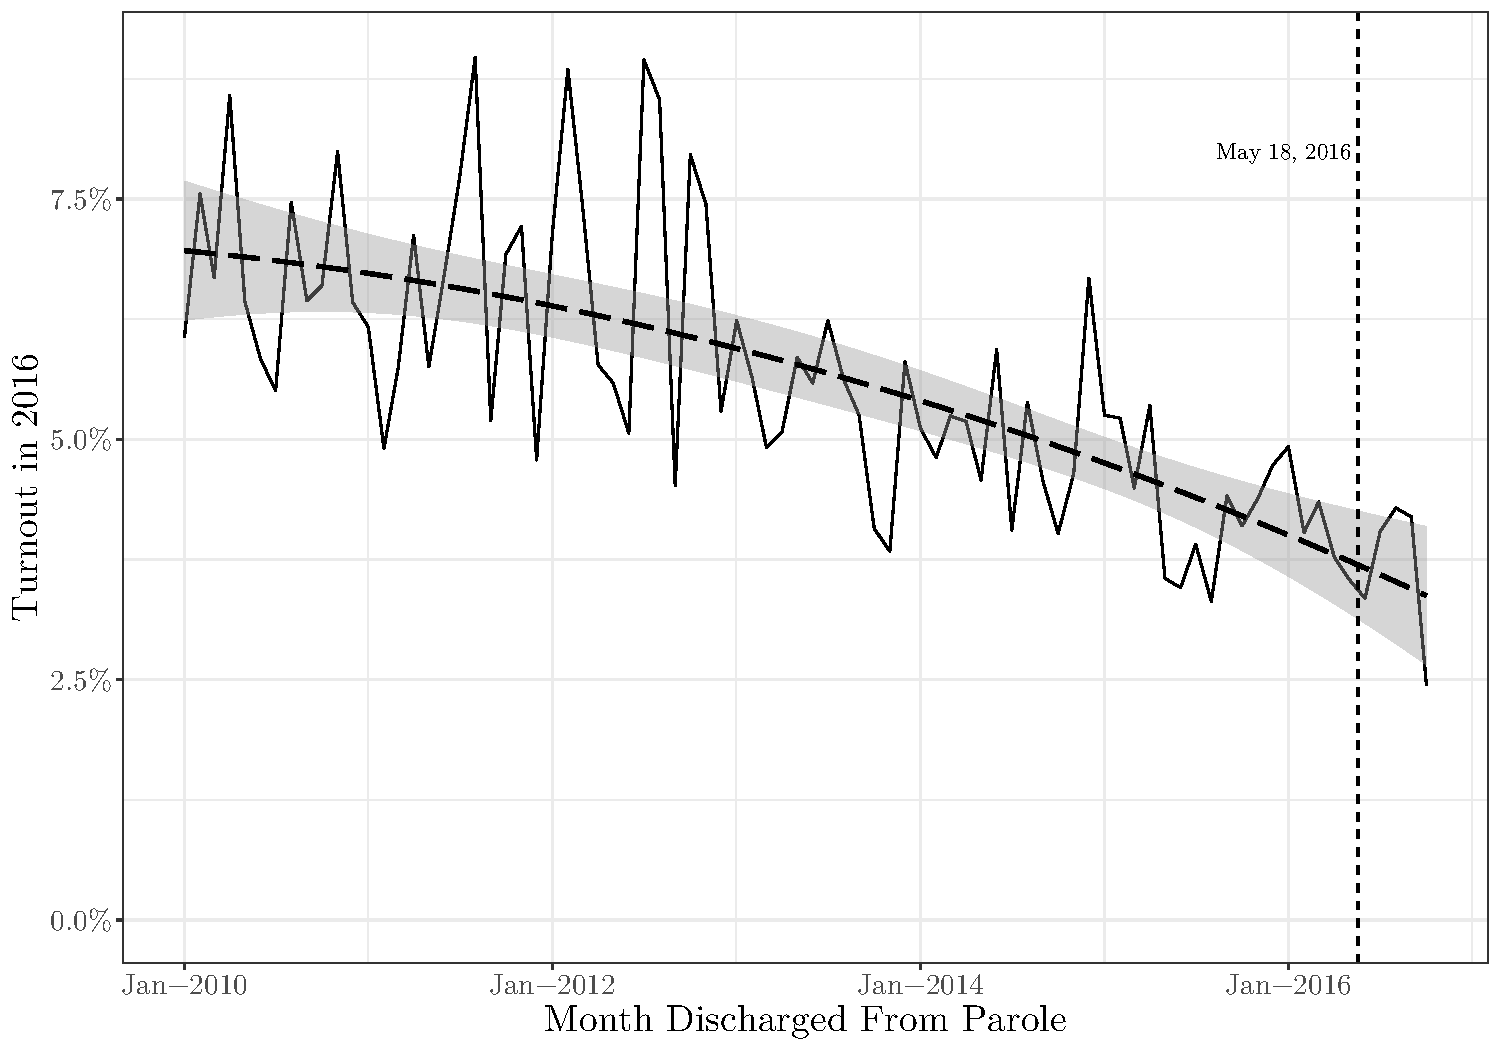
\includegraphics[width=0.85\linewidth,height=0.85\textheight]{mpsa_files/figure-beamer/unnamed-chunk-1-1} \end{center}
\end{frame}

\begin{frame}{Turnout in 2018 Among the Formerly Incarcerated}
\protect\hypertarget{turnout-in-2018-among-the-formerly-incarcerated}{}
\begin{center}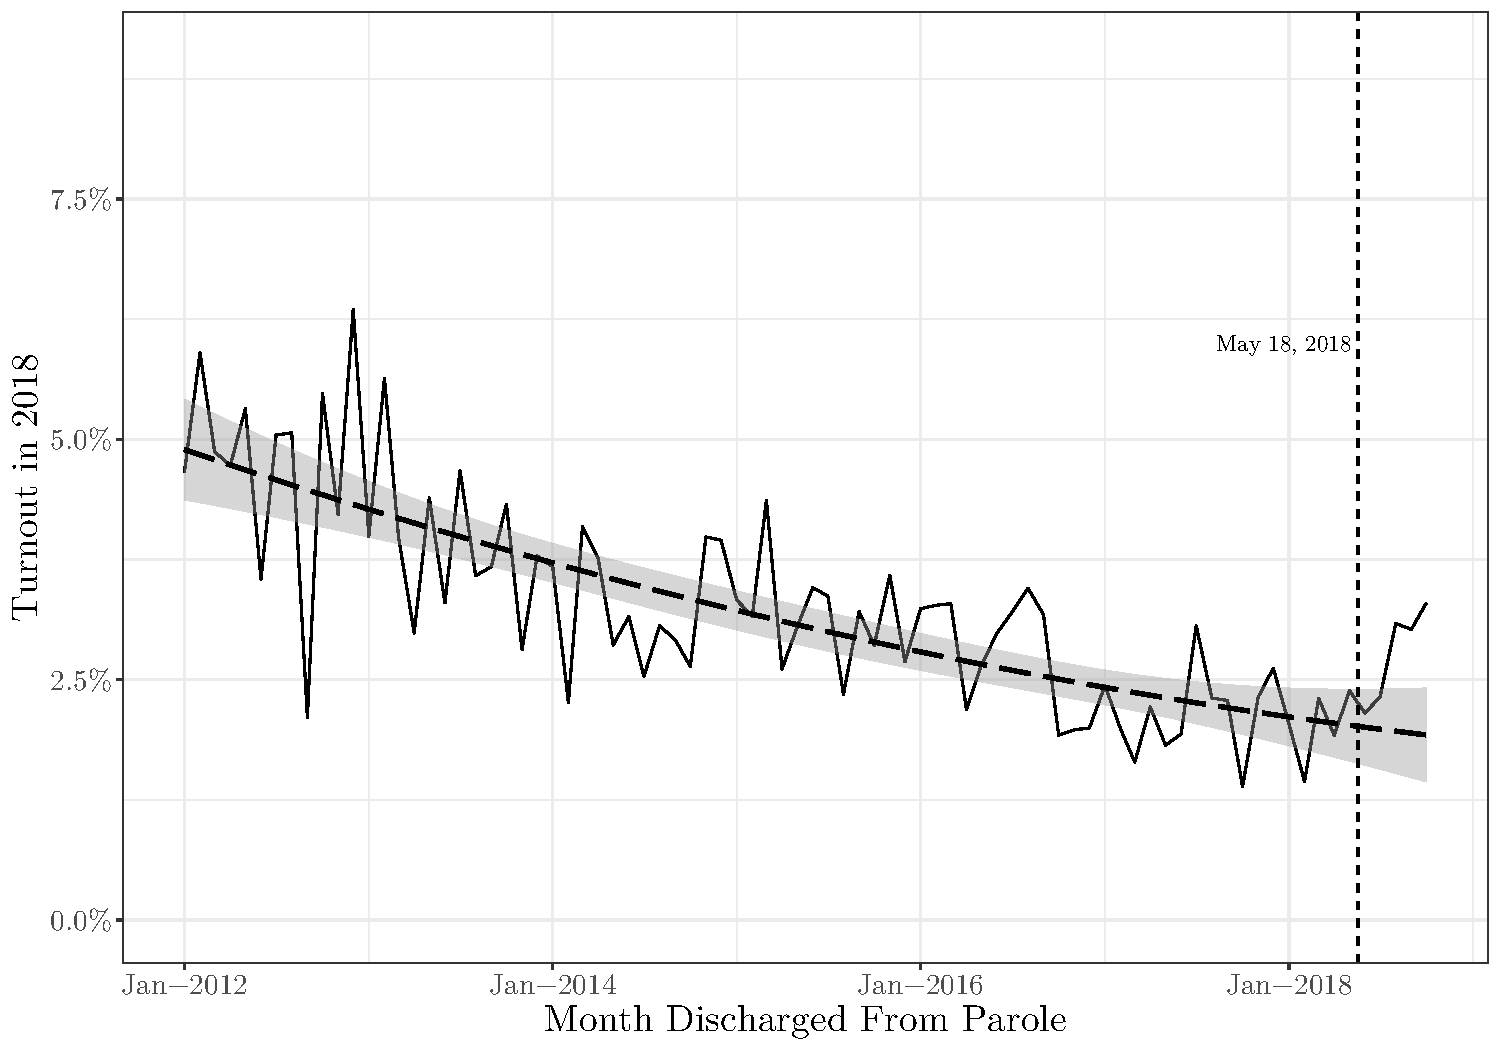
\includegraphics[width=0.85\linewidth,height=0.85\textheight]{mpsa_files/figure-beamer/unnamed-chunk-2-1} \end{center}
\end{frame}

\begin{frame}{Overall Treatment Effects}
\protect\hypertarget{overall-treatment-effects}{}
\begin{center}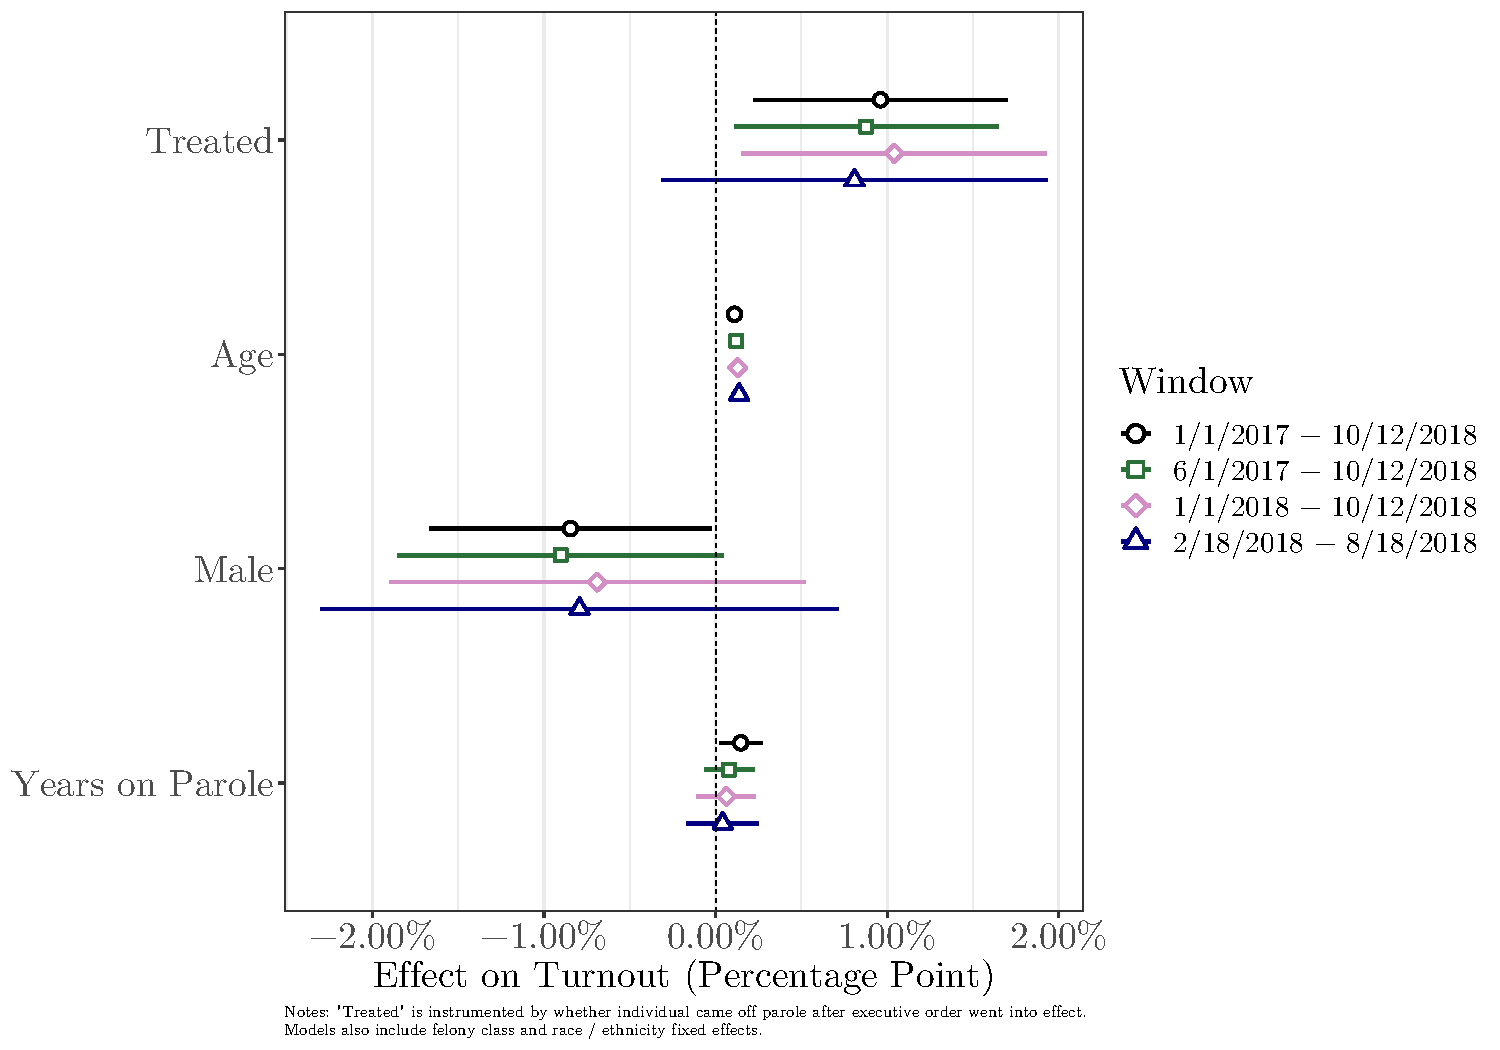
\includegraphics[width=0.85\linewidth,height=0.85\textheight]{mpsa_files/figure-beamer/unnamed-chunk-3-1} \end{center}
\end{frame}

\begin{frame}{Treatment Effects Vary by Race}
\protect\hypertarget{treatment-effects-vary-by-race}{}
\begin{center}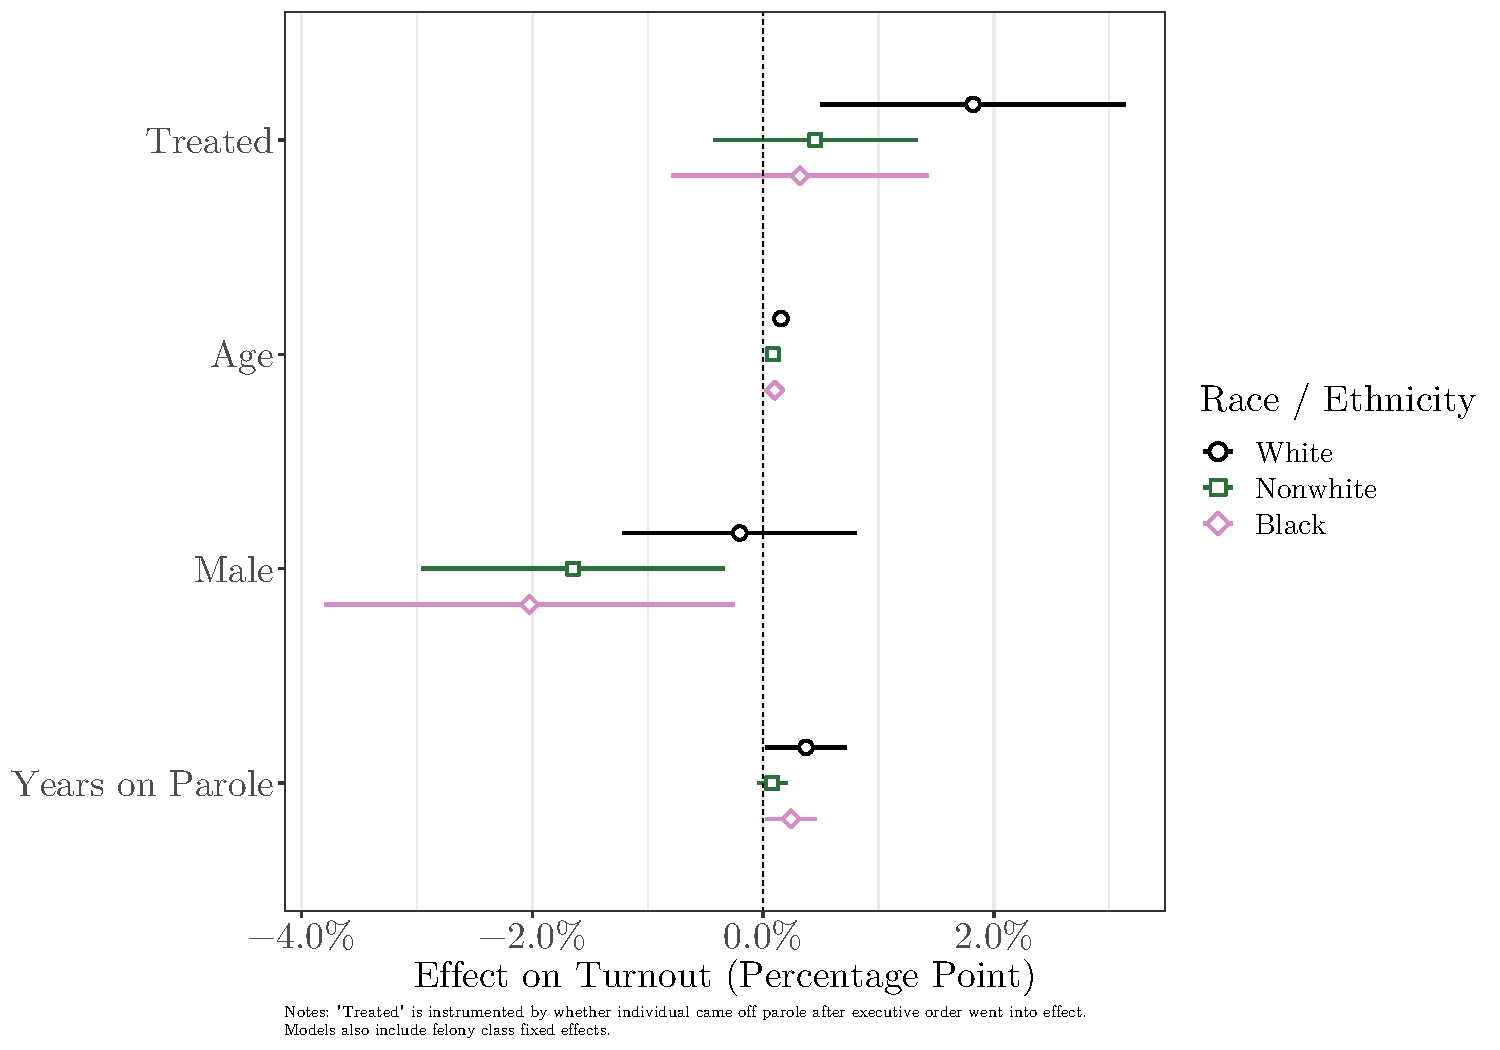
\includegraphics[width=0.85\linewidth,height=0.85\textheight]{mpsa_files/figure-beamer/unnamed-chunk-4-1} \end{center}
\end{frame}

\begin{frame}{We Made It!}
\protect\hypertarget{we-made-it}{}
Thanks!

\href{mailto:kevin.morris@nyu.edu}{\nolinkurl{kevin.morris@nyu.edu}}
\end{frame}

\begin{frame}[allowframebreaks,allowframebreaks]{References}
\protect\hypertarget{references}{}
\hypertarget{refs}{}
\begin{cslreferences}
\leavevmode\hypertarget{ref-Burch2011}{}%
Burch, Traci. 2011. ``Turnout and Party Registration Among Criminal
Offenders in the 2008 General Election.'' \emph{Law \& Society Review}
45 (3): 699--730.
\url{https://doi.org/10.1111/j.1540-5893.2011.00448.x}.

\leavevmode\hypertarget{ref-Burch2012}{}%
---------. 2012. ``Did Disfranchisement Laws Help Elect President Bush?
New Evidence on the Turnout Rates and Candidate Preferences of Florida's
Ex-Felons.'' \emph{Political Behavior} 34 (1): 1--26.
\url{https://doi.org/10.1007/s11109-010-9150-9}.

\leavevmode\hypertarget{ref-Gerber2015}{}%
Gerber, Alan S., Gregory A. Huber, Marc Meredith, Daniel R. Biggers, and
David J. Hendry. 2015. ``Can Incarcerated Felons Be (Re)Integrated into
the Political System? Results from a Field Experiment.'' \emph{American
Journal of Political Science} 59 (4): 912--26.
\url{https://doi.org/10.1111/ajps.12166}.

\leavevmode\hypertarget{ref-Gerber2017}{}%
---------. 2017. ``Does Incarceration Reduce Voting? Evidence About the
Political Consequences of Spending Time in Prison.'' \emph{The Journal
of Politics} 79 (4): 1130--46. \url{https://doi.org/10.1086/692670}.

\leavevmode\hypertarget{ref-Lerman2014}{}%
Lerman, Amy E., and Vesla M. Weaver. 2014. \emph{Arresting Citizenship:
The Democratic Consequences of American Crime Control}. Chicago Studies
in American Politics. Chicago ; London: The University of Chicago Press.

\leavevmode\hypertarget{ref-Meredith2015}{}%
Meredith, Marc, and Michael Morse. 2015. ``The Politics of the
Restoration of Ex-Felon Voting Rights: The Case of Iowa.''
\emph{Quarterly Journal of Political Science} 10 (1): 41--100.
\url{https://doi.org/10.1561/100.00013026}.

\leavevmode\hypertarget{ref-White2019}{}%
White, Ariel. 2019. ``Misdemeanor Disenfranchisement? The Demobilizing
Effects of Brief Jail Spells on Potential Voters.'' \emph{American
Political Science Review} 113 (2): 311--24.
\url{https://doi.org/10.1017/S000305541800093X}.
\end{cslreferences}
\end{frame}

\end{document}
